\ifx\PREAMBLE\UnDef
\documentclass{beamer}
\usepackage{tikz}
\usetikzlibrary{snakes,arrows}

\usepackage[english]{babel}
% or whatever

\usepackage[latin1]{inputenc}
% or whatever

\usepackage[T1]{fontenc}
\usepackage{amssymb}
\usepackage{amsmath}
\usepackage{eventB}

\begin{document}
\else
\fi


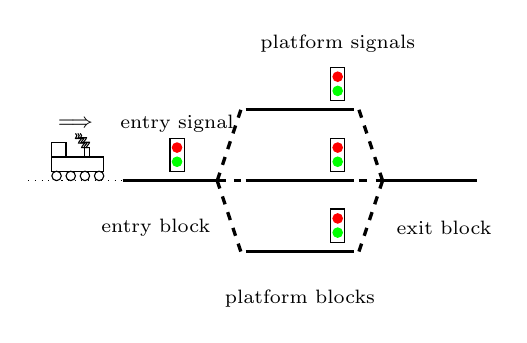
\begin{tikzpicture}[scale=0.6]
  \scriptsize
  % approaching block.
  \draw[very thick] (0,0) -- (1.5,0);
  \draw (0.7, -1) node{entry block};

  % in-switch
  \draw[very thick] (1.5,0) -- (2,0);
  \draw[very thick, dashed] (2,0) -- (2.5,1.5);
  \draw[very thick, dashed] (2,0) -- (2.5,-1.5);
  \draw[very thick, dashed] (2,0) -- (2.5,0);
%  \draw[red] (2, -1.5) node{in-switch};
  
  % platform blocks
  \draw[very thick] (2.6,0) -- (4.9,0);
%  \draw[very thick, dotted] (2.6,0.5) -- (4.9,0.5);
%  \draw[very thick, dotted] (2.6,-0.5) -- (4.9,-0.5);
  \draw[very thick] (2.6,1.5) -- (4.9,1.5);
  \draw[very thick] (2.6,-1.5) -- (4.9,-1.5);
  \draw (3.75, -2.5) node{platform blocks};

  % out-switch
  \draw[very thick] (5.5,0) -- (6,0);
  \draw[very thick, dashed] (5,1.5) -- (5.5,0);
  \draw[very thick, dashed] (5,0) -- (5.5,0);
  \draw[ very thick, dashed] (5,-1.5) -- (5.5,0);
%  \draw[red] (5.5, -1.5) node{out-switch};

  % exiting block.
  \draw[very thick] (6.0,0) -- (7.5,0);
  \draw (6.8, -1) node{exit block};

  % entry signal
%  \draw[very thick] (1.45,0) -- (1.45, 1);
  \draw (1, 0.2) rectangle +(0.3,0.7);
  \filldraw[red] (1.15, 0.7) circle (0.1);
  \filldraw[green] (1.15, 0.4) circle (0.1);
  \draw (1.15, 1.2) node{entry signal};

  % platform signals
%  \draw[very thick] (6.05,0) -- (6.05, 1);
  \draw (4.4, 0.2) rectangle +(0.3,0.7);
  \filldraw[red] (4.55, 0.7) circle (0.1);
  \filldraw[green] (4.55, 0.4) circle (0.1);
  \draw (4.55, 2.9) node{platform signals};

  \draw (4.4, 1.7) rectangle +(0.3,0.7);
  \filldraw[red] (4.55, 2.2) circle (0.1);
  \filldraw[green] (4.55, 1.9) circle (0.1);

  \draw (4.4, -1.3) rectangle +(0.3,0.7);
  \filldraw[red] (4.55, -0.8) circle (0.1);
  \filldraw[green] (4.55, -1.1) circle (0.1);

  % The train
  \draw[dotted] (-2,0) -- (0, 0);
  \draw(-1.5,0.2) rectangle +(1.1, 0.3);
  \draw(-1.5,0.5) rectangle +(0.3, 0.3);
  \draw(-0.8,0.5) rectangle +(0.1, 0.2);
  \draw[decorate, decoration={snake, amplitude = 1pt, segment length = 2pt}] (-0.8,0.7) --  (-1,1);
  \draw[decorate, decoration={snake, amplitude = 1pt, segment length = 2pt}] (-0.75,0.7) --  (-0.95,1);
  \draw[decorate, decoration={snake, amplitude = 1pt, segment length = 2pt}] (-0.7,0.7) --  (-0.9,1);
  \draw (-1.4, 0.1) circle (0.1);
  \draw (-1.1, 0.1) circle (0.1);
  \draw (-0.8, 0.1) circle (0.1);
  \draw (-0.5, 0.1) circle (0.1);
  \draw (-1, 1.2) node{$\Longrightarrow$};
\end{tikzpicture}

\ifx\PREAMBLE\UnDef
\end{document}
\else
\fi
